% !TeX encoding=utf8
% !TeX spellcheck = de_CH_frami

\section*{Abstract}

%Praktisches Beispiel einer Prozess-Steuerung im Bereich Home-Automation
\subsection*{Ausgangslage und Ziel}
Die Seminararbeit "`Praktisches Beispiel einer Prozesssteuerung im Bereich Home Automation"' soll zeigen, was es heute für Möglichkeiten gibt um Prozesse und Abläufe im Bereich Home Automation und BPM (Business Process Management) zu automatisieren. Dabei soll ein End-to-End Beispiel auf einem Raspberry Pi implementiert werden.

\subsection*{Vorgehensweise}
Im Rahmen der Arbeit wird zuerst der aktuelle Stand von BPM im Kontext IOT (Internet of Things) und anschliessend im Bereich "`Home Automation"' betrachtet. Aufgrund der Erkenntnisse aus diesen Bereichen wird anschliessend analysiert, was es für Möglichkeiten gibt Prozesse und Abläufe auf einem Raspberry Pi im Kontext "`Home Automation"' zu realisieren. Im Anschluss wird mit einer ausgewählten Lösung ein Beispielprozess implementiert.

\subsection*{Der Setup und der realisierte Beispielprozess}
Als Beispiel wurde ein "`Türlinkgel-Prozess"' realisiert. Dieser Prozess wird ausgelöst, wenn an der Haustüre geklingelt wird. Innerhalb des Prozesses werden verschiedene Kriterien (Ist zu Hause, Ist in den Ferien) ausgewertet und je nach Zustand ein anderer Prozesszweig durchlaufen. Für die Realisierung wurde ein Raspberry Pi 2 mit einem Razberry Z-Wave Board, eine Z-Wave LED Glühbirne und ein Z-Wave Wandschalter verwendet. Softwareseitig wurden folgende Komponenten verwendet: Mosquitto MQTT Broker, ejabberd XMPP Server, Apache Derby Database, H2 Database, Apache Tomcat 7, activiti BPM Platform, Postfix Mail Server und openHAB 2 als Home Automation Lösung.

\begin{figure}[H]
  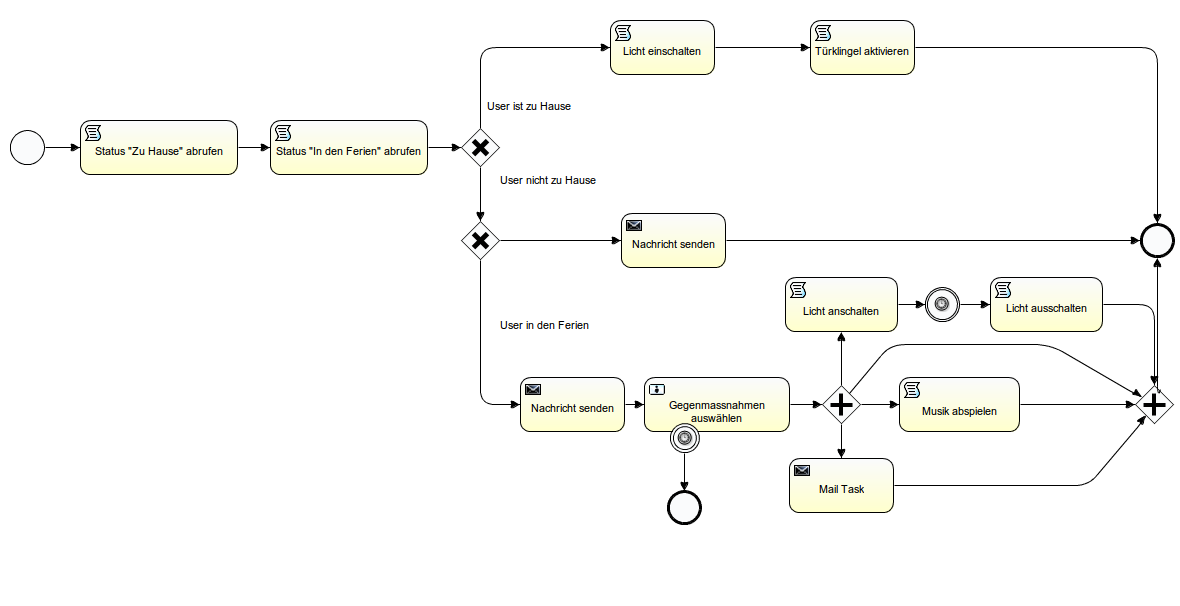
\includegraphics[width=14cm]{./images/DoorBellProcess}  \caption{"'Türklingel-Prozess"'}\label{img:AnalyseRpi:DoorbellProcess}
\end{figure}
